	\newpage
\section{Projektowanie}		%3
%Opis przygotowania narzędzi (git, visual studio). Wybór i opis bibliotek, klas. Szkic layoutów. Pseudo kody. Opisy wykorzystanych algorytmów (np. algorytm sortowania). Dokładniejsze określenie założeń i działania aplikacji, (np.: ten przycisk otworzy takie okno a w tym oknie wpisujemy takie dane).

\subsection{Przygotowanie narzędzi Git oraz Visual Studio}

\hspace{1cm}W celu korzystania z narzędzia Git należy utworzyć na swoim komputerze repozytorium lokalne oraz dodać do niego pliki projektu. Na platformie GitHub utworzyć repozytorium zdalne, które umożliwi wszystkim autorom projektu współprace przy tworzeniu aplikacji.
\newline
W Visual Studio należy zainstalować dodatek opracowywanie aplikacji mobilnych za pomocą środowiska Xamarin oraz zestaw Android SDK, który umożliwia korzystanie z emulatora.
Do tworzenia projeku wybraliśmy szablon aplikacji mobilnej Xamarin.Forms.
Xamarin.Forms ma duży ekosystem bibliotek, które dodają różne funkcje do aplikacji. W tej sekcji opisano niektóre z tych dodatkowych funkcji\footnote{https://docs.microsoft.com/pl-pl/xamarin/get-started/what-is-xamarin-forms\cite{www1}.}.

\subsection{Biblioteki i klasy}
\hspace{1cm} \textbf{Biblioteka Xamarin.Essentials} udostępnia międzyplatformowy interfejs programowania aplikacji mobilnych (API). Jest ona dostępna jako pakiet NuGet i jest uwzględniana w każdym nowym projekcie w programie Visual Studio.
Biblioteka ta oferuje klasy, które zostaną przez nas użyte podczas tworzenia projektu\footnote{https://docs.microsoft.com/pl-pl/xamarin/essentials/?context=xamarin/xamarin-forms\cite{www2}.}.
\newline
\textbf{Geolokalizacja:}
\newline
\textbf{Klasa Geolocation} udostępnia interfejsy API do pobierania bieżących współrzędnych geolokalizacji urządzenia.
\newline
\textbf{Motyw aplikacji:}
\newline
Interfejs API RequestedTheme jest częścią klasy AppInfo i zawiera informacje dotyczące tematu żądanego dla uruchomionej aplikacji przez system.
\newline
\textbf{Akcelerometr:}
\newline
\textbf{Klasa Accelerometer} umożliwia monitorowanie czujnika przyspieszeniomierza urządzenia, który wskazuje przyspieszenie urządzenia w trójwymiarowej przestrzeni.
\newline
\textbf{GoogleMap:}
\newline
Firma Google oferuje natywny interfejs API mapowania dla systemu Android. Pozwala on na zmienianie punktu widzenia mapy, dodawanie i dostosowywanie znaczników, oznaczanie mapy za pomocą nakładek.
\newline
Wymagania wstępne Mapy API usługi Google: uzyskanie klucza Mapy API, zainstalowanie pakietu Xamarin.GooglePlayServices i Mapy pakietu z NuGet, określenie wymaganych uprawnień.
\newline
\textbf{Klasa GoogleMaps} poprzez aplikację platformy Xamarin.Android będzie współdziałała z aplikacją Google Maps.
\newline
\newline
\textbf{Biblioteka Microsoft Authentication Library (MSAL)} pozwala na dodawanie uwierzytelniania do aplikacja. Umożliwi to logowanie do aplikacji przy użyciu Google lub Facebook.
\newline
\textbf{Klasa WebAuthenticator} umożliwia inicjowanie przepływów opartych na przeglądarce, które nasłuchują wywołania zwrotnego do określonego adresu URL zarejestrowanego w aplikacji.
\newline

\subsection{Layouty dla opcji z menu}
Po wybraniu z menu opcji \textbf{Mapa} na ekranie wyświetli się mapa pokazująca przebytą trasę oraz zaznaczająca miejsce w którym użytkownik w danym momencie się znajduje co jest pokazane na rysunku 3.1.
Na mapie będą się także wyświetlały zdjęcia miejsc docelowych zrobione przez użytkownika.
\begin{figure}[!htb]
	\begin{center}
		\includegraphics[width=10cm]{rys/Mapa.png}
		\caption{Layout - Mapa}
		\label{rys:rysunek003}
	\end{center}
\end{figure}
\newline Opcja \textbf{Wyniki} wyświetli stronę zawierającą wyniki z ostatnich 7 dni oraz najlepszy wynik z całej historii. Wśród wyświetlanych wyników znajdą się: Przybyta odległość, liczba kroków oraz liczba spalonych kalorii jak na rysunku 3.2. Pozwoli to użytkownikowi na porównywanie swoich wyników oraz zmotywuje do poprawiania rekordowych wyników.
\begin{figure}[!htb]
	\begin{center}
		\includegraphics[width=8cm]{rys/Wyniki.png}
		\caption{Layout - Wyniki}
		\label{rys:rysunek004}
	\end{center}
\end{figure}
\newline Wybór opcji \textbf{Zdjęcia} otworzy galerie zdjęć wykonanych przez użytkownika jak na rysunku 3.3. Zdjęcia będą przedstawiać miejsca docelowe uwiecznione aparatem telefonu.
\begin{figure}[!htb]
	\begin{center}
		\includegraphics[width=6cm]{rys/Zdjęcia.png}
		\caption{Layout - Zdjęcia}
		\label{rys:rysunek005}
	\end{center}
\end{figure}
\newline
\newline Opcja \textbf{Wybierz} normę pozwala na wybranie dystansu jaki użytkownik planuje przebyć w ciągu dnia. Polega to na zaznaczeniu checkboxa obok wybranej odległości zo jest widoczne na rysunku 3.4.
\begin{figure}[!htb]
	\begin{center}
		\includegraphics[width=8cm]{rys/Wybierz.png}
		\caption{Layout - Wybierz normę}
		\label{rys:rysunek006}
	\end{center}
\end{figure}
 
 \subsection{Stworzenie pliku apk na Androida z poziomu Visual Studio}
 \hspace{1cm}Aby umożliwić stworzenie pliku apk w Visual Studio należy wejść w właściwości rozwiązania dla systemu Android.Następnie w opcjach systemu Android trzeba odznaczyć opcję \textbf{Użyj udostępnionego środowiska uruchomieniowego} jak na rysunku 3.5.
 \begin{figure}[!htb]
 	\begin{center}
 		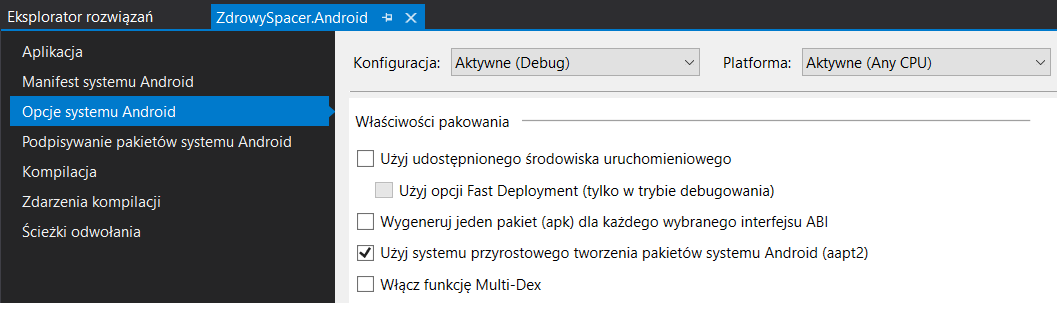
\includegraphics[width=12cm]{rys/apk_1.png}
 		\caption{Odznaczenie właściwości w Opcjach systemu Android}
 		\label{rys:rysunek007}
 	\end{center}
 \end{figure}
 \newline Na rysunku 3.6 widzimy, że kolejny krok to Archiwizacja rozwiązania dla systemu Android
 \begin{figure}[!htb]
 	\begin{center}
 		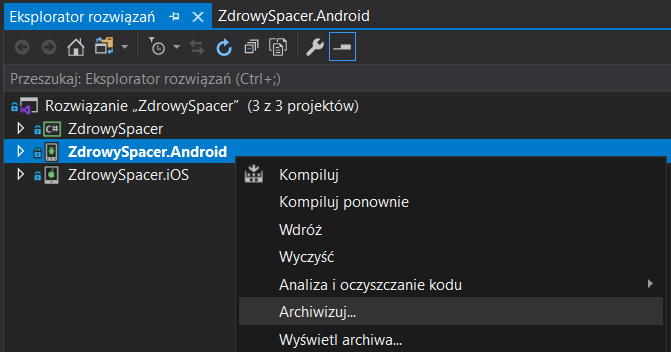
\includegraphics[width=12cm]{rys/apk_2.png}
 		\caption{Archiwizacja rozwiązania dla systemu Android}
 		\label{rys:rysunek008}
 	\end{center}
 \end{figure}
 \newline W \textbf{Menedżer archiwów} należy wybrać wersje aplikacji i nacisnąć przycisk \textbf{Dystrybuuj...} jak na rysunku 3.7.
 \begin{figure}[!htb]
 	\begin{center}
 		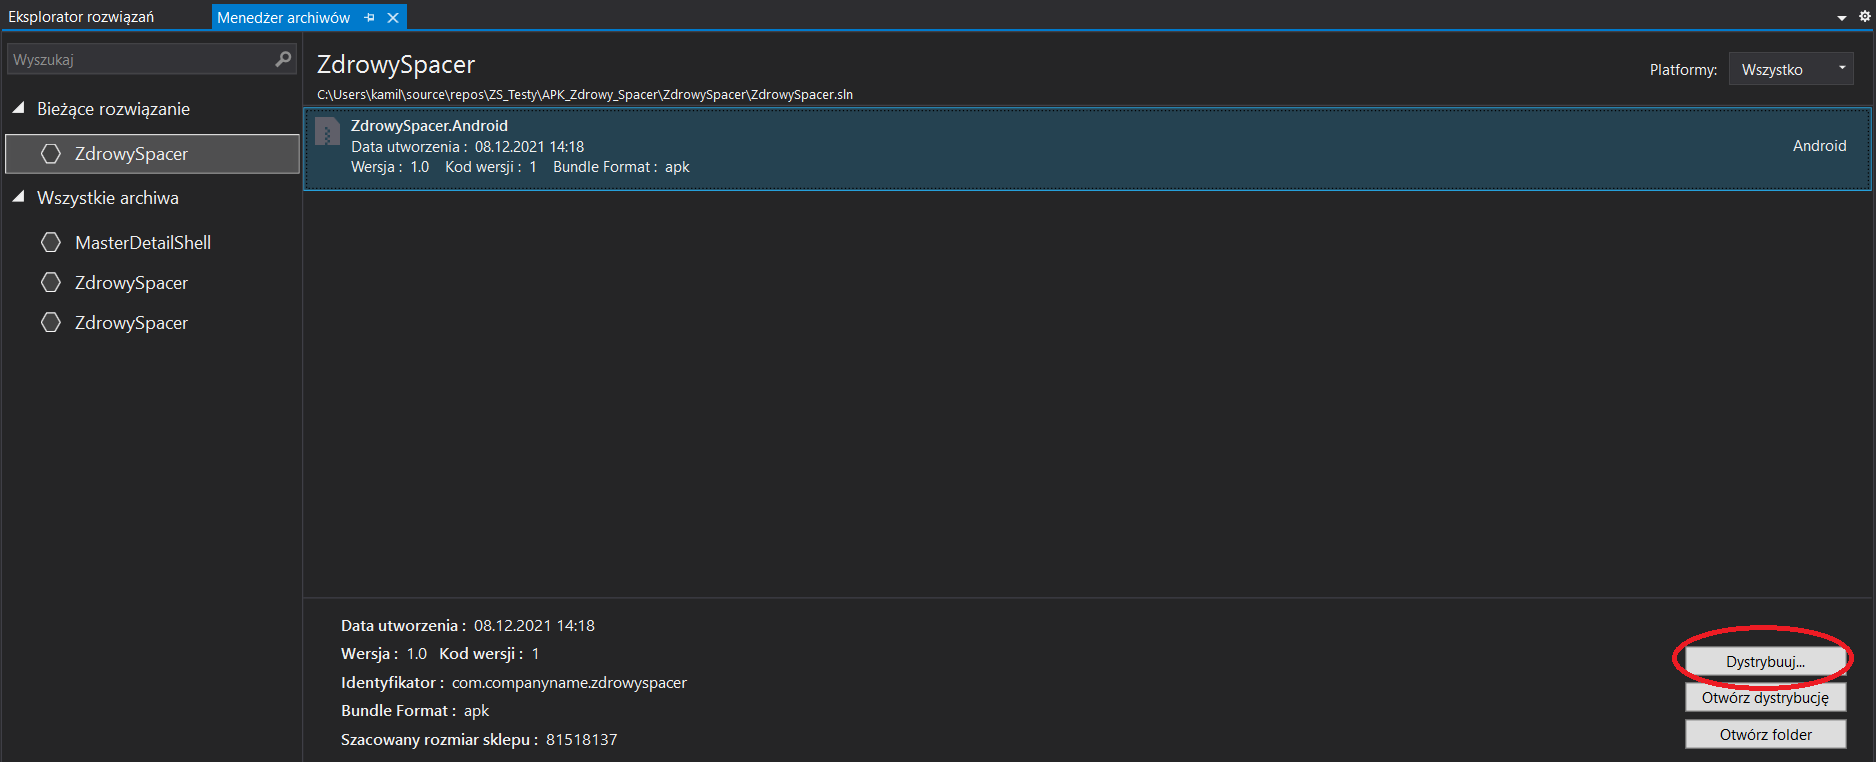
\includegraphics[width=12cm]{rys/apk_3.png}
 		\caption{Dystrybucja pliku}
 		\label{rys:rysunek009}
 	\end{center}
 \end{figure}
\newpage
 Na rysunku 3.8 zaprezentowano wybór kanału dystrybucji jako opcji \textbf{Ad Hoc}
 \begin{figure}[!htb]
 	\begin{center}
 		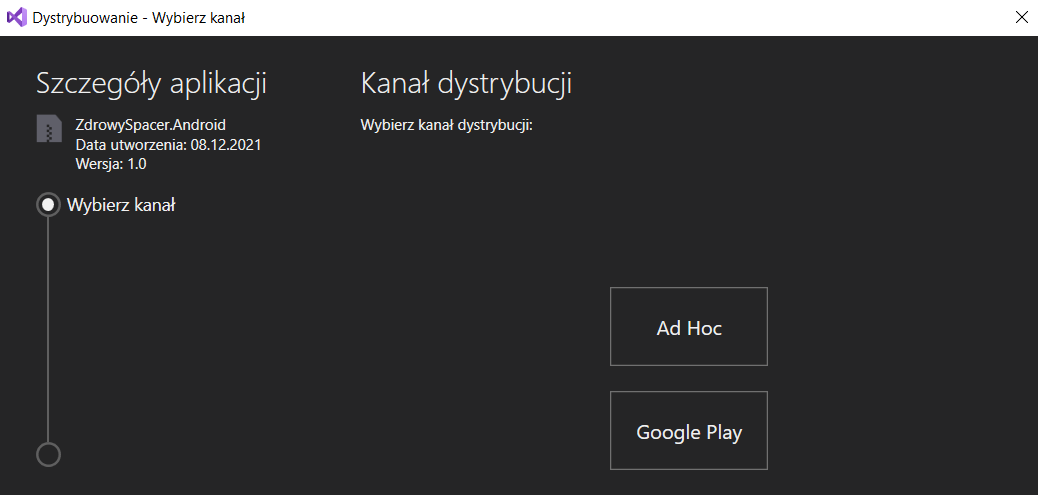
\includegraphics[width=12cm]{rys/apk_4.png}
 		\caption{Wybranie kanału dystrybucji}
 		\label{rys:rysunek010}
 	\end{center}
 \end{figure}
 \newline Ostatni krok to podpisanie pliku za pomocą wcześniej utworzonego aliasu jak widać na rysunku 3.9 i wybranie miejsca w którym chcemy zapisać plik apk
 \begin{figure}[!htb]
 	\begin{center}
 		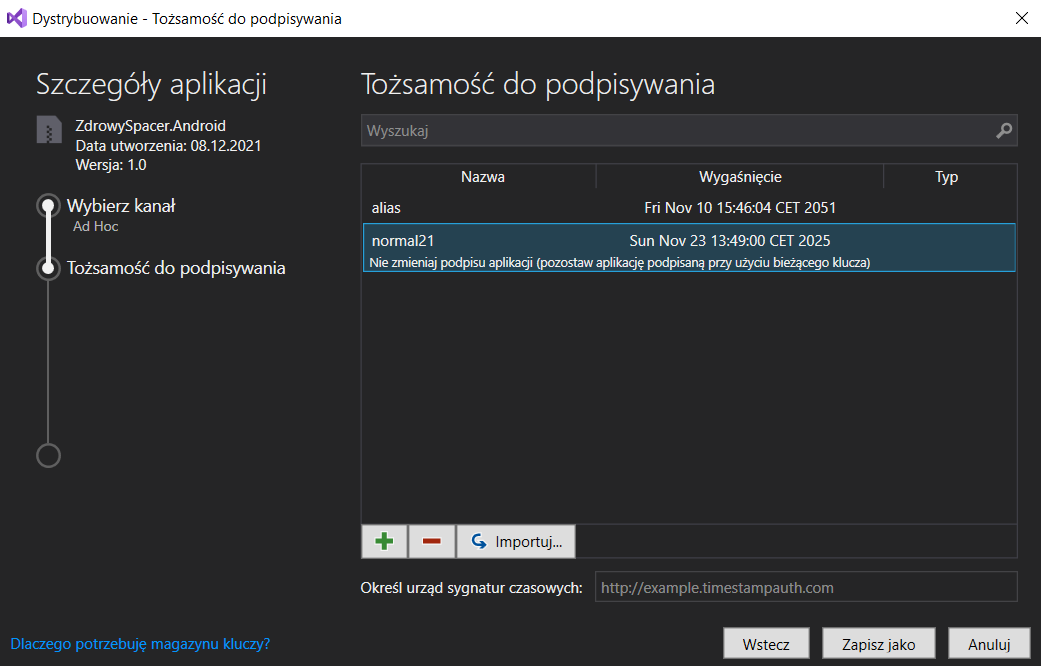
\includegraphics[width=12cm]{rys/apk_5.png}
 		\caption{Podpis za pomocą aliasu}
 		\label{rys:rysunek011}
 	\end{center}
 \end{figure}
 